
%% bare_conf.tex
%% V1.4b
%% 2015/08/26
%% by Michael Shell
%% See:
%% http://www.michaelshell.org/
%% for current contact information.
%%
%% This is a skeleton file demonstrating the use of IEEEtran.cls
%% (requires IEEEtran.cls version 1.8b or later) with an IEEE
%% conference paper.
%%
%% Support sites:
%% http://www.michaelshell.org/tex/ieeetran/
%% http://www.ctan.org/pkg/ieeetran
%% and
%% http://www.ieee.org/

%%*************************************************************************
%% Legal Notice:
%% This code is offered as-is without any warranty either expressed or
%% implied; without even the implied warranty of MERCHANTABILITY or
%% FITNESS FOR A PARTICULAR PURPOSE! 
%% User assumes all risk.
%% In no event shall the IEEE or any contributor to this code be liable for
%% any damages or losses, including, but not limited to, incidental,
%% consequential, or any other damages, resulting from the use or misuse
%% of any information contained here.
%%
%% All comments are the opinions of their respective authors and are not
%% necessarily endorsed by the IEEE.
%%
%% This work is distributed under the LaTeX Project Public License (LPPL)
%% ( http://www.latex-project.org/ ) version 1.3, and may be freely used,
%% distributed and modified. A copy of the LPPL, version 1.3, is included
%% in the base LaTeX documentation of all distributions of LaTeX released
%% 2003/12/01 or later.
%% Retain all contribution notices and credits.
%% ** Modified files should be clearly indicated as such, including  **
%% ** renaming them and changing author support contact information. **
%%*************************************************************************


% *** Authors should verify (and, if needed, correct) their LaTeX system  ***
% *** with the testflow diagnostic prior to trusting their LaTeX platform ***
% *** with production work. The IEEE's font choices and paper sizes can   ***
% *** trigger bugs that do not appear when using other class files.       ***                          ***
% The testflow support page is at:
% http://www.michaelshell.org/tex/testflow/



\documentclass[conference]{IEEEtran}
% Some Computer Society conferences also require the compsoc mode option,
% but others use the standard conference format.
%
% If IEEEtran.cls has not been installed into the LaTeX system files,
% manually specify the path to it like:
% \documentclass[conference]{../sty/IEEEtran}





% Some very useful LaTeX packages include:
% (uncomment the ones you want to load)


% *** MISC UTILITY PACKAGES ***
%
%\usepackage{ifpdf}
% Heiko Oberdiek's ifpdf.sty is very useful if you need conditional
% compilation based on whether the output is pdf or dvi.
% usage:
% \ifpdf
%   % pdf code
% \else
%   % dvi code
% \fi
% The latest version of ifpdf.sty can be obtained from:
% http://www.ctan.org/pkg/ifpdf
% Also, note that IEEEtran.cls V1.7 and later provides a builtin
% \ifCLASSINFOpdf conditional that works the same way.
% When switching from latex to pdflatex and vice-versa, the compiler may
% have to be run twice to clear warning/error messages.






% *** CITATION PACKAGES ***
%
%\usepackage{cite}
% cite.sty was written by Donald Arseneau
% V1.6 and later of IEEEtran pre-defines the format of the cite.sty package
% \cite{} output to follow that of the IEEE. Loading the cite package will
% result in citation numbers being automatically sorted and properly
% "compressed/ranged". e.g., [1], [9], [2], [7], [5], [6] without using
% cite.sty will become [1], [2], [5]--[7], [9] using cite.sty. cite.sty's
% \cite will automatically add leading space, if needed. Use cite.sty's
% noadjust option (cite.sty V3.8 and later) if you want to turn this off
% such as if a citation ever needs to be enclosed in parenthesis.
% cite.sty is already installed on most LaTeX systems. Be sure and use
% version 5.0 (2009-03-20) and later if using hyperref.sty.
% The latest version can be obtained at:
% http://www.ctan.org/pkg/cite
% The documentation is contained in the cite.sty file itself.






% *** GRAPHICS RELATED PACKAGES ***
%
\ifCLASSINFOpdf
  % \usepackage[pdftex]{graphicx}
  % declare the path(s) where your graphic files are
  % \graphicspath{{../pdf/}{../jpeg/}}
  % and their extensions so you won't have to specify these with
  % every instance of \includegraphics
  % \DeclareGraphicsExtensions{.pdf,.jpeg,.png}
\else
  % or other class option (dvipsone, dvipdf, if not using dvips). graphicx
  % will default to the driver specified in the system graphics.cfg if no
  % driver is specified.
  % \usepackage[dvips]{graphicx}
  % declare the path(s) where your graphic files are
  % \graphicspath{{../eps/}}
  % and their extensions so you won't have to specify these with
  % every instance of \includegraphics
  % \DeclareGraphicsExtensions{.eps}
\fi
% graphicx was written by David Carlisle and Sebastian Rahtz. It is
% required if you want graphics, photos, etc. graphicx.sty is already
% installed on most LaTeX systems. The latest version and documentation
% can be obtained at: 
% http://www.ctan.org/pkg/graphicx
% Another good source of documentation is "Using Imported Graphics in
% LaTeX2e" by Keith Reckdahl which can be found at:
% http://www.ctan.org/pkg/epslatex
%
% latex, and pdflatex in dvi mode, support graphics in encapsulated
% postscript (.eps) format. pdflatex in pdf mode supports graphics
% in .pdf, .jpeg, .png and .mps (metapost) formats. Users should ensure
% that all non-photo figures use a vector format (.eps, .pdf, .mps) and
% not a bitmapped formats (.jpeg, .png). The IEEE frowns on bitmapped formats
% which can result in "jaggedy"/blurry rendering of lines and letters as
% well as large increases in file sizes.
%
% You can find documentation about the pdfTeX application at:
% http://www.tug.org/applications/pdftex





% *** MATH PACKAGES ***
%
%\usepackage{amsmath}
% A popular package from the American Mathematical Society that provides
% many useful and powerful commands for dealing with mathematics.
%
% Note that the amsmath package sets \interdisplaylinepenalty to 10000
% thus preventing page breaks from occurring within multiline equations. Use:
%\interdisplaylinepenalty=2500
% after loading amsmath to restore such page breaks as IEEEtran.cls normally
% does. amsmath.sty is already installed on most LaTeX systems. The latest
% version and documentation can be obtained at:
% http://www.ctan.org/pkg/amsmath





% *** SPECIALIZED LIST PACKAGES ***
%
%\usepackage{algorithmic}
% algorithmic.sty was written by Peter Williams and Rogerio Brito.
% This package provides an algorithmic environment fo describing algorithms.
% You can use the algorithmic environment in-text or within a figure
% environment to provide for a floating algorithm. Do NOT use the algorithm
% floating environment provided by algorithm.sty (by the same authors) or
% algorithm2e.sty (by Christophe Fiorio) as the IEEE does not use dedicated
% algorithm float types and packages that provide these will not provide
% correct IEEE style captions. The latest version and documentation of
% algorithmic.sty can be obtained at:
% http://www.ctan.org/pkg/algorithms
% Also of interest may be the (relatively newer and more customizable)
% algorithmicx.sty package by Szasz Janos:
% http://www.ctan.org/pkg/algorithmicx




% *** ALIGNMENT PACKAGES ***
%
%\usepackage{array}
% Frank Mittelbach's and David Carlisle's array.sty patches and improves
% the standard LaTeX2e array and tabular environments to provide better
% appearance and additional user controls. As the default LaTeX2e table
% generation code is lacking to the point of almost being broken with
% respect to the quality of the end results, all users are strongly
% advised to use an enhanced (at the very least that provided by array.sty)
% set of table tools. array.sty is already installed on most systems. The
% latest version and documentation can be obtained at:
% http://www.ctan.org/pkg/array


% IEEEtran contains the IEEEeqnarray family of commands that can be used to
% generate multiline equations as well as matrices, tables, etc., of high
% quality.




% *** SUBFIGURE PACKAGES ***
%\ifCLASSOPTIONcompsoc
%  \usepackage[caption=false,font=normalsize,labelfont=sf,textfont=sf]{subfig}
%\else
%  \usepackage[caption=false,font=footnotesize]{subfig}
%\fi
% subfig.sty, written by Steven Douglas Cochran, is the modern replacement
% for subfigure.sty, the latter of which is no longer maintained and is
% incompatible with some LaTeX packages including fixltx2e. However,
% subfig.sty requires and automatically loads Axel Sommerfeldt's caption.sty
% which will override IEEEtran.cls' handling of captions and this will result
% in non-IEEE style figure/table captions. To prevent this problem, be sure
% and invoke subfig.sty's "caption=false" package option (available since
% subfig.sty version 1.3, 2005/06/28) as this is will preserve IEEEtran.cls
% handling of captions.
% Note that the Computer Society format requires a larger sans serif font
% than the serif footnote size font used in traditional IEEE formatting
% and thus the need to invoke different subfig.sty package options depending
% on whether compsoc mode has been enabled.
%
% The latest version and documentation of subfig.sty can be obtained at:
% http://www.ctan.org/pkg/subfig




% *** FLOAT PACKAGES ***
%
%\usepackage{fixltx2e}
% fixltx2e, the successor to the earlier fix2col.sty, was written by
% Frank Mittelbach and David Carlisle. This package corrects a few problems
% in the LaTeX2e kernel, the most notable of which is that in current
% LaTeX2e releases, the ordering of single and double column floats is not
% guaranteed to be preserved. Thus, an unpatched LaTeX2e can allow a
% single column figure to be placed prior to an earlier double column
% figure.
% Be aware that LaTeX2e kernels dated 2015 and later have fixltx2e.sty's
% corrections already built into the system in which case a warning will
% be issued if an attempt is made to load fixltx2e.sty as it is no longer
% needed.
% The latest version and documentation can be found at:
% http://www.ctan.org/pkg/fixltx2e


%\usepackage{stfloats}
% stfloats.sty was written by Sigitas Tolusis. This package gives LaTeX2e
% the ability to do double column floats at the bottom of the page as well
% as the top. (e.g., "\begin{figure*}[!b]" is not normally possible in
% LaTeX2e). It also provides a command:
%\fnbelowfloat
% to enable the placement of footnotes below bottom floats (the standard
% LaTeX2e kernel puts them above bottom floats). This is an invasive package
% which rewrites many portions of the LaTeX2e float routines. It may not work
% with other packages that modify the LaTeX2e float routines. The latest
% version and documentation can be obtained at:
% http://www.ctan.org/pkg/stfloats
% Do not use the stfloats baselinefloat ability as the IEEE does not allow
% \baselineskip to stretch. Authors submitting work to the IEEE should note
% that the IEEE rarely uses double column equations and that authors should try
% to avoid such use. Do not be tempted to use the cuted.sty or midfloat.sty
% packages (also by Sigitas Tolusis) as the IEEE does not format its papers in
% such ways.
% Do not attempt to use stfloats with fixltx2e as they are incompatible.
% Instead, use Morten Hogholm'a dblfloatfix which combines the features
% of both fixltx2e and stfloats:
%
% \usepackage{dblfloatfix}
% The latest version can be found at:
% http://www.ctan.org/pkg/dblfloatfix




% *** PDF, URL AND HYPERLINK PACKAGES ***
%
\usepackage{url}
% url.sty was written by Donald Arseneau. It provides better support for
% handling and breaking URLs. url.sty is already installed on most LaTeX
% systems. The latest version and documentation can be obtained at:
% http://www.ctan.org/pkg/url
% Basically, \url{my_url_here}.




% *** Do not adjust lengths that control margins, column widths, etc. ***
% *** Do not use packages that alter fonts (such as pslatex).         ***
% There should be no need to do such things with IEEEtran.cls V1.6 and later.
% (Unless specifically asked to do so by the journal or conference you plan
% to submit to, of course. )



% correct bad hyphenation here
\hyphenation{op-tical net-works semi-conduc-tor}


\usepackage{graphicx}
\begin{document}
%
% paper title
% Titles are generally capitalized except for words such as a, an, and, as,
% at, but, by, for, in, nor, of, on, or, the, to and up, which are usually
% not capitalized unless they are the first or last word of the title.
% Linebreaks \\ can be used within to get better formatting as desired.
% Do not put math or special symbols in the title.
% TODO Make the title more interesting and informative of the contribution
\title{Pathfinding with Obstacle Avoidance\\Using Fuzzy Logic}


% author names and affiliations
% use a multiple column layout for up to three different
% affiliations
\author{\IEEEauthorblockN{Jelle van Dijk}
\IEEEauthorblockA{
University of Amsterdam\\
Student ID: 10989048
}
\and
\IEEEauthorblockN{Gawan Dekker}
\IEEEauthorblockA{
University of Amsterdam\\
Student ID: 11025654
}
\and 
\IEEEauthorblockN{Victor Gladys}
\IEEEauthorblockA{
University of Amsterdam\\
Student ID: 10523626
}
}

\date{}


% make the title area
\maketitle

% As a general rule, do not put math, special symbols or citations
% in the abstract
\begin{abstract}
The abstract goes here (to be done later).
\end{abstract}

% For peer review papers, you can put extra information on the cover
% page as needed:
% \ifCLASSOPTIONpeerreview
% \begin{center} \bfseries EDICS Category: 3-BBND \end{center}
% \fi
%
% For peerreview papers, this IEEEtran command inserts a page break and
% creates the second title. It will be ignored for other modes.
\IEEEpeerreviewmaketitle



% TODO Provide references in the introduction. Your starting point is very interesting, but give a brief overview of the approaches taken to the problem.
\section{Introduction}
Self driving cars are being developed at almost every major car and tech company in the world right now. Although they are still relatively early in development, they are considered by many to be the future of personal transportation. To try and gain a better understanding of autonomous moving vehicles, in this project we attempt to recreate a simple one using a fuzzy logic system (FLS).\\
% TODO The goal should be related to the problem, not the solution. This is the place where you briefly mention the existing approaches to the problem of autonomous navigation. It is a very well studied problem and it is quite rich in resources.
The goal of this project is to create and design a FLS that can guide a robot through different environments without colliding with any obstacles. Because of limited time and recourses we have not implemented this system for an actual vehicle or robot, instead, we worked with a simulation. Both the FLS and the simulation are created by ourselves. We then applied our FLS to our simulated robot in place of an obstacle avoidance algorithm.
%Both the FLS and the simulation will be written in python. The environment and obstacles will be represented in a number of grids. The simulated robot will get a starting position in this grid and a position as the target to be moving towards.
% TODO These implementation details should be given in the proposed approach section. Use introduction as a medium for warming up to the problem, giving references, elaborate more on your motivation, objectives, limitations and scope etc.


% TODO Do not subsection the references, just give brief take-away points of the previous work, do not summarise it.
\section{Literature Review}
There is already a lot of literature about trying to make a robot traverse an environment using fuzzy logic. In this section, we will briefly discuss three papers that are relevant to our problem.

%\subsection{Artificial Neural Fuzzy Logic Algorithm for Robot Path Finding (X. Bajrami; A. D\"ermaku; N. Demaku)}
In ``Artificial Neural Fuzzy Logic Algorithm for Robot Path Finding'' \cite{bajrami2015artificial}, X. Bajrami, A. D\"ermaku and N. Demaku create and compare two fuzzy logic implementations to guide a robot from point A to point B in a simulated environment with obstacles.\\
The first implementation uses a combination of FLSs with mamdani-type inferrence and handmade rulebases and membership functions to guide the robot. The input (distances to closest objects and goal, angle towards goal and preferred turn) is used to determine acceleration levels for the left and right wheels of the robot for different objectives (like obstacle avoidance) and to determine different weights for those objectives.\\
The second implementation used an FLS with a Sugeno-type inference system, where the membership functions were trained using a neuro-adaptive learning method.\\
After running tests in a simulated environment, the two implementations were compared.\\
The first implementation in the paper comes close to what we have implemented. We have used the the distance to obstacles in three different directions as inputs to give information about the area the robot is moving towards. And give two angles of rotation, one to the left and one to the right, as outputs. These are combined to create a single rotation angle.
% We are using similar input, although (for the time being) we use one FLS with an incomplete rulebase to guide the robot.
% TODO Use an academic language and give scientific justifications.

% TODO Punctuation, language and spell check needed.
%\subsection{A Novel Hybrid Fuzzy A* Robot Navigation System for Target Pursuit and Obstacle Avoidance (A. P. Gerdelan; Dr. N. H. Reyes, Ph.D.)}
In ``A Novel Hybrid Fuzzy A* Robot Navigation
System for Target Pursuit and Obstacle Avoidance'' \cite{gerdelan2006novel}, the researcher created a hybrid system to control a robot. The first layer of the system consisted of an A* algorithm. The A* algorithm is a path finding algorithm, it is considered to be very fast. The A* path finding layer calculated the optimal route to from the position of the robot to the end point, this route consisted of way points. The second layer of the system is a fuzzy logic system. This system had as input information about the next way point as well as about the nearest obstacle. With these pieces of information a speed and turning speed for the robot were chosen.\\
This paper used some techniques that can be very useful for our project. Since they used a moving end point in their simulations, their test scenarios where harder. However, the same principles they used to control their robot will apply to the robot in the simulations used in our project.\\
One problem that the researchers in \cite{gerdelan2006novel} encountered, was that in some situation the fuzzy logic system would try to avoid an obstacle and by doing so, would not be able to move to the next way point. This is something to keep in mind for our project, but could be fixed by tweaking the membership functions.
% TODO I think you would need a more intelligent way, such as a hierarchical system to implement such behaviour. 

%\subsection{Adaptive two layer fuzzy control of a mobile robot system (M. Mohammadian; R. J. Stonier)}
In ``Adaptive two layer fuzzy control of a mobile robot system'' \cite{mohammadian1995adaptive}, a genetic algorithm has been used to adapt fuzzy rules in a two layer fuzzy logic system, which is then used by two robots to navigate towards a target without colliding.
The genetic learning has been applied to generate a new layer of fuzzy rules that can be integrated into an already existing rulebase.\\
The first of the two fuzzy layers is used to determine the angle at which to continue moving, whilst the second layer determines the speed of the robot. By encoding the rulebase into a bitstring, Mohammadian \textit{et al.} were able to modify the rulebases with a genetic algorithm using cross-over and single-point mutations over a number of generations. To do this they used a modified cross-over procedure that ensured that these bitstrings were cut only at points that defined boundaries between rules.\\
The paper concludes in noting that, altough most of their tests resulted in a positive outcome, some had trouble at the corners of the tested driving areas. This suggests that genetic algorithms find a maximum in optimizing fuzzy systems that is not necessarily easily applicable to a change in, or extension of, the initial learning environment.
% TODO Use the related work as an inspiration to your approach and provide what you will be doing differently. Elaborate more on: What will you contribute? What was the shortcoming of the previous systems? Be critical. 

\section{Proposed Approach}
% TODO If you do not have data to learn from you may skip this section. In the design, you can emphasize that the system is based on expert knowledge.
%\subsection{Data}
%Most of the data will be personal knowledge. The first versions of membership functions and rules will be created by us. When possible the newer versions of the membership functions and rules will be extrapolated from the test result of the previous evolution of the system.
\subsection{Design}
%The general design of our system is still unknown at this point. As inputs we will use the distances to the nearest objects at several degrees of rotation and the distance and angle to the target location. As outputs, we will use accelleration and degree of rotation of the robot. However, these might all still be subject to change.
Our Fuzzy Logic System uses three inputs and gives two outputs. The inputs we use are the distance to the nearest object in three different directions: front, front-left and front-right. The output is given in the form of two angles a left angle and a right angle, the robot will move in the direction of the combination of these two angles.\\
Our input variables have a mix of triangular and trapezoidal membership functions (
%TODO figures of memberships functions
). For all three inputs the range (in pixels) and membership functions are equal. The placement of the functions is chosen such that only a very small distance (about the size of the robot) is seen as a small distance, anything above about 5x the robots size is seen as a large distance and in between is a medium amount of distance. The functions have a reasonable amount of overlap since the random obstacle movement in our environment is cause for a decent amount of overlap.\\
We use a full rulebase of 27 rules for our system (
%TODO table with rules
). In general, the rules are chosen such that the robot makes sharper turns if the distance to the objects in front of it is smaller and will always prioritize a left turn over a right turn.\\

\subsection{Implementation}
%The two most important parts, the simulation and the Fuzzy Logic System, will be created by us in python (exact algorithms are not yet known).
We used python to build both the Fuzzy Logic System implementation and the simulated environment. For the simulations we primarily used the pygame package.\\
\subsubsection{Fuzzy Logic System implementation}
We implemented a variety of possible membership functions for our FLS implementation. Most of which use standard functions to return membership. For the triangular and trapezoidal membership functions, however, we used a sequence of if-else statements to calculate membership, rather than taking the minimum value from two lines. This way it was easier to make sure we do not accidentally devide by zero.\\
For our input and output variables, we simply record a name, range and list of membership functions. When calculating the membership, we return a dictionary with all memberships of a datapoint for the membership functions of the variable.\\
For our rules, we implemented AND and OR rules. AND rules can be calculated using the minimum operation or the algebraic product. OR rules can be calculated using the max operation or the algebraic sum.\\
% TODO inference/aggregation/defuzzification with pseudocode
\subsubsection{Simulated Environment}
The environment our robot moves around in is a box with an amount of obstacles. The obstacles are rectangular in shape and move in a random direction. Every certain amount of timesteps, the direction in which the obstacles move changes in a random new direction.\\
The robot moves around in this environment at a fixed speed and has to avoid colliding with the obstacles. The change in angle of the robot at every tick is determined by the FLS.\\
The distance from the robot to an object are determined by raycasting. For each timestep, the robot casts two rays slightly around the desired direction. With this ray, the distance to the nearest object (that includes the walls of the simulation) is determined. The distance in that direction is then the smallest value returned from those two rays. This is done for angles around 0 degrees, 35 degrees and -35 degrees and the distances are passed to the FLS. The FLS then determines a left and right turning degree and the middle of those two angles is taken as the change in directions that the robot follows.
% TODO maybe pseudocode
% TODO Link to repo?
\subsection{Link to repository}
% TODO remove underscores from directory and url
\url{https://gitlab-fnwi.uva.nl/10989048/fuzzy_logic_final_project}
\url{https://github.com/Yelvd/Fuzzy_logic_final_project}

\section{Experiments and Results}
A starting situation was created for the simulation. This starting situation consisted of the robot in the corner at the bottom left and 14 square obstacles of varying sizes placed around the field, see figure~\ref{fig:start}.

\begin{figure}[!ht]
  \centering
  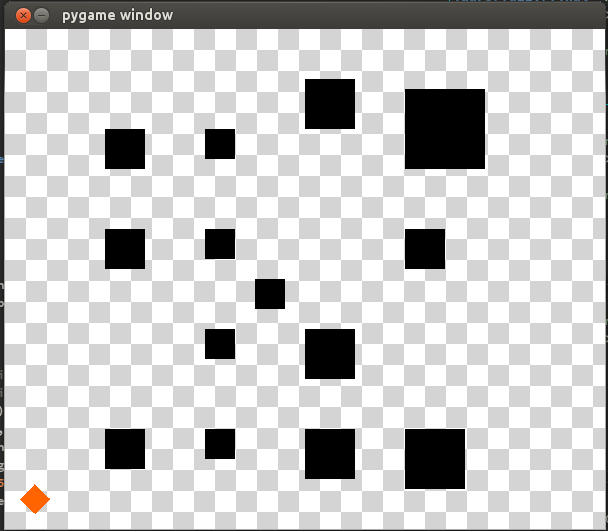
\includegraphics[scale=0.3]{./figs/StartSetup.png}
  \caption{starting situation for the simulation}
  \label{fig:start}
\end{figure}

\noindent
The obstacle move each in there own random direction, after 30 frames they pick a new random direction. When colliding with an other object or the wall the obstacle rotate there direction vector 45 degrees clockwise each frame until they can move again. A simulation terminates when the robot collides with an obstacle or the wall. The data that was collected is the length of a simulation in frames.
Frames where chosen as measurement unit instead of time since this allows us to speed up our simulations by unlocking the number of frames per second, the data is also more reliable because it is changed if the computer the experiment is run on cannot keep up with the simulation.\\

The following sets of speeds where chosen:
\begin{itemize}
  \item Player: 2 pixels/frame, Obstacle: 1 pixels/frame
  \item Player: 2 pixels/frame, Obstacle: 2 pixels/frame
  \item Player: 2 pixels/frame, Obstacle: 4 pixels/frame
  \item Player: 6 pixels/frame, Obstacle: 6 pixels/frame
\end{itemize}

\noindent
For each set of speeds two different types of terminate conditions where used. The first one being that the simulation terminates if the player makes a move that result in a collision with either an obstacle or the wall, on the other test the simulation terminated when the player collided with an obstacle or wall or when an obstacle made a move that resulted in a collision. For each set of speeds both termination conditions where run 20 times. The average frames until termination is reported below.

\subsection{Results}

\section{Discussion}

%TODO
%\section{Conclusions and Future Work}
%The conclusion goes here (to be done later).




% conference papers do not normally have an appendix


% use section* for acknowledgment
% \section*{Acknowledgment}

% TODO Use more and diverse references to self-driving cars.
\nocite{*}
\bibliographystyle{IEEEtranS}
\bibliography{mybibfile}


% that's all folks
\end{document}
